\documentclass[14pt]{extarticle}

\title{A Preprint \\ <<Повышение пространственного разрешения спутниковых данных с применением нейронных сетей для определения характеристик лесных пород>>.\\[5mm]\large Выполнил: Валеев Арслан Рустамович\\ студент 417 группы ММП ВМК МГУ.\\[5mm]\large Научный руководитель: к.ф-м.н., доцент\\ Гуров Сергей Исаевич}
% \author{Валеев Арслан Рустамович}

\date{декабрь 2024.}

\usepackage[warn]{mathtext}
\usepackage[T2A]{fontenc}
\usepackage[utf8]{inputenc}
\usepackage[english,russian]{babel}
\usepackage{indentfirst}
\usepackage{csquotes}
\usepackage{wrapfig}
\usepackage{extsizes}
\usepackage{svg}
\usepackage{unicode-math}
\usepackage{array}
\usepackage{biblatex}
% \usepackage[
% backend=biber,
% style=alphabetic,
% ]{biblatex}
\addbibresource{cites.bib}

\usepackage[
     left=1.8cm,
     right=1.8cm,
     top=1.8cm,
     bottom=1.8cm,
     bindingoffset=0cm,
]{geometry}

\usepackage{graphicx, hyperref, xcolor}
\hypersetup{
    colorlinks=true,
    linkcolor=teal,
    filecolor=magenta,
    urlcolor=blue,
    citecolor=olive,
    pdftitle={GD},
    linktoc=all
}

\usepackage{caption}
\usepackage{subcaption}
\usepackage{floatrow}
\floatsetup{heightadjust=object}

\usepackage{amsmath, amsfonts, amssymb,amsthm, mathtools, esint, eucal}

\begin{document}
\maketitle
\tableofcontents


\section{Постановка задачи}
Целью данной работы является сравнение производительности нескольких SR архитектур: ESRGAN, SwinIR, ESRGAN+LDL на имеющемся наборе данных. Эти архитектуры используют разные подходы для генерации изображений высокого разрешения. Основыне задачи исследования:
\begin{itemize}
    \item Подготовка набора данных: выбрать лучший способ загрубления и аугментации данных для спутниковых снимков
    \item Реализация и обучение моделей: обучение архитектур ESRGAN,\\ ESRGAN+LDL, SwinIR на наборе данных с целью повышения пространственного разрешения изображений.
    \item Анализ гиперпараметров: оценка влияния различных параметров и разработок (варьирование лосса) на обобщающую способность модели.
\end{itemize}
\section{Введение}

В настоящее время использование спутниковых данных для мониторинга и анализа объектов и явлений в окружающей среде становится все более распространенным и актуальным. Однако получение изображений высокого качества требует значительных ресурсов и использования высокотехнологичного оборудования. Кроме того, существует проблема передачи данных между различными устройствами, которые могут работать с разными допустимыми разрешениями изображений. Именно в связи с этими проблемами возникает потребность в разработке эффективных методов повышения пространственного разрешения изображений. Рассмотрим более подробно, почему нейронные сети становятся необходимыми для решения этой задачи и почему стандартные методы, такие как линейная или бикубическая интерполяция, могут быть недостаточно эффективными.


\subsection{Введение в область super resolution}
Далее используются обозначения:
\begin{itemize}
    \item LR (image) - изображение низкого разрешения
    \item HR (image) - изображение высокого разрешения
    \item SR (image) - восстановленное изображение высокого разрешения из изображения низкого разрешения
\end{itemize}

% $M(i, j) = \left\{\begin{matrix}
%  0,&  if \ | R(i, j) |< |R_s(i, j)|\\ 
%  \delta\cdot  S(i, j),& if \ | R(i, j) |\geqslant  |R_s(i, j)|
% \end{matrix}\right.$

В основном, сейчас все методы повышения разрешения можно грубо поделить на два направления:\textit{ Single Image Super Resolution} (SISR) и \textit{Multi Image Super Resolution} (MISR). В SISR стоит задача реконструкции HR изображения по одному экземпляру LR. В MISR дано несколько LR снимков одной локации, по которым нужно восстановить HR изображение этой же локации. Хотя задача MISR имеет больше априорной информации (благодаря снимкам с разных ракурсов можно восстановить большую часть высокочастотной информации), но в реальных задачах, зачастую сложно получить несколько разных снимков одной и той же локации. Поэтому далее работа будет посвящена SISR. В этой сфере, задача реконструкции изображения поставлена некорректно - в LR изображении может потеряться часть высокочастотной информации, которая может быть восстановлена/дополнена множеством способов - корректных решений у изображения множество, и все они по-своему правильные. 
% Далее будет рассмотрен подход, генерирующий по LR распределение соответствующих ему HR изображений, тем самым частично решая проблему недетерменированности решения.


В SISR методы преимущественно делятся на два семейства - Interpolation-based и Reconstruction-based.

Interpolation-based - это интерполяция изображений методами nearest neighbors, bicubic, bilinear e.t.c. эти методы вычисляют значения пикселей нового изображения, используя расположенные в окрестности пиксели LR снимка. Эти алгоритмы довольно быстрые, но не в состоянии восстановить высокочастотные детали изображения.


Reconstruction-based использует априорную информацию в домене, чтобы задать ограничения на генерацию HR изображения. Известные алгоритмы этого семейства - проекция на выпуклые множества (POCS) \cite{PROCS},
maximum-a-posteriori (MAP) \cite{MAP} подход. К этому семейству относится большинство нейросетевых алгоритмов.


\subsection{Интуиция стоящая за нейросетевыми алгоритмами}

Пусть рассматривается произвольное изображение $P$, тогда количество информации на нем обозначается как $I(P)$. В контексте алгоритмической трансформации (интерполяции) $Tr(.)$, справедливо, что $I(P) => I(Tr(P))$. Иными словами, любое детерминированное преобразование не увеличивает количество информации на изображении. Это открывает двери для применения нейронных сетей, которые способны <<генерировать>> или, можно сказать, <<галлюцинировать>> дополнительную информацию на изображениях, опираясь на закономерности, выявленные в тренировочных данных. Это позволяет нейронным сетям эффективно повышать разрешение изображений, что является критически важным в сфере анализа спутниковых данных.


\subsection{Обзор методов в рассматриваемой области}
На сегодняшний день существует несколько нейросетевых подходов к решению задачи SISR (Single Image Super-Resolution). Среди них \textbf{CNN-based} подход, использующий свёрточные нейронные сети в своей архитектуре. Первые шаги в этом направлении были сделаны в статье \cite{DL2015}, предложившей архитектуру SRCNN. Далее была разработана модель SRResNet, использующая Residual connections, которая является адаптацией модели ResNet для задачи SISR. Данная модель активно используется исследователями в качестве бейзлайна или базовой архитектуры для более продуктивных решений.

\subsubsection{CNN-based подходы}
Из недавних работ в этой сфере можно выделить архитектуру WindSR \cite{WindSR}, основанную на SRResNet, где residual blocks заменены на Residual-in-Residual Dense Blocks. Данная архитектура применялась для повышения пространственного разрешения карты скорости ветра. Данные были взяты из датасета GEOS-5 Nature Run с разрешением 7 км на ячейку сетки и бикубической интерполяцией понижались до 28 км на ячейку сетки для получения низкого разрешения (LR) изображений. Авторам удалось достичь прироста 11.35\% в метрике RMSE по сравнению с передовыми GAN-методами.


Архитектура SRS3 \cite{SRS3} использует механизм внимания для выделения наиболее информативных каналов в картах признаков. В качестве данных использовались снимки Sentinel-2 с MSI сенсором для получения высокоразрешённых (HR) изображений и Sentinel-3 с OLCI сенсором для низкоразрешённых (LR) изображений. Авторам удалось достичь прироста +0.33 dB для увеличения разрешения в 2 раза по сравнению с SRCNN.

Работа SARNet \cite{SARNet} использует SRResNet с добавлением channel-attention механизма в блоки residual connections. Модель обучалась на данных с Sentinel-2 с разрешением 10 м и данных спутника PlanetScope с разрешением 5 м и 2.5 м.

\subsubsection{Generative-based подходы}

Данный подход предполагает обучение генератора и дискриминатора для создания изображений высокого разрешения (HR) и их классификации соответственно. GAN (Generative Adversarial Networks) широко используется в SISR, так как способен генерировать больше мелких деталей по сравнению с CNN-based подходами, которые преимущественно сглаживают изображение. Первопроходцем считается архитектура SRGAN \cite{SRGAN}, однако часто используется ESRGAN \cite{wang2018esrgan}, улучшенная версия SRGAN, использующая relativistic discriminator.

Интересна работа \cite{unplannedUrban}, где SRGAN применялся для улучшения качества сегментации незарегистрированного населения в городах Китая. Данные брались со спутников GaoFen-2 (1 м) и Sentinel-2 (10 м). Авторам удалось добиться улучшения качества сегментации по метрике IoU более чем в два раза по сравнению с изображениями низкого разрешения, что сопоставимо с оригинальными изображениями.

Также стоит отметить работу \cite{EASR}, использующую SRGAN архитектуру с EASR модулем, который использует градиент реконструированного изображения для улучшения генерации деталей. Это позволило улучшить качество сегментации на 10\% по метрике IoU.

Отдельно можно отметить работу \cite{LDL2022}, в которой был представлен LDL модуль, улучшающий качество изображений путём штрафования модели за генерацию артефактов. Модуль тестировался на датасетах DIV2K и DF2K, но в \cite{SAGAN} он используется для спутниковых изображений GaoFen-2 и GaoFen-7.

\subsubsection{Transformer-based подходы}

Transformer-based подходы позволяют более эффективно переводить изображения в формат высокого разрешения. В работах \cite{Liang2021SwinIRIR, SwinIR+CNN} представлены две модели. В первой из них предложена SOTA модель SwinIR использующая Swin, а во второй предложено объединение CNN-based и Transformer-based подходов с использованием легковесных моделей.

\subsubsection{Diffusion models}

Диффузионные модели активно используются для SISR благодаря своей способности генерировать визуально более приятные изображения, чем другие SOTA решения \cite{SR3, SRDiff}. Однако в сфере спутниковых изображений они начали применяться относительно недавно из-за низкой скорости инференса модели. Среди примеров можно выделить модели DMDC \cite{DMDC} и EDiffSR \cite{EDiffSR}.

% \subsubsection{CNN-based}
% На сегодняшний день существует несколько нейросетевых подходов к решению задачи SISR. Среди них \textbf{CNN-based} подход, использующий свёртки в своей архитектуре. Первые шаги в этом направлении были сделаны в статье \cite{DL2015}, подарившей нам архитектуру SRCNN. Далее была предоставлена модель SRResNet[4], которая использовала Residual connections в своей архитектуре, и по сути, была адаптацией модели ResNet под задачу SISR. Данная модель активно используется исследователями в качестве бейзлайна, или в качестве базовой архитектуры, на основе которой можно предоставить более продуктивное решение. Из недавних работ в этой сфере можно выделить архитектуру WindSR \cite{WindSR}, основанная на SRResNet, с заменой residual blocks на ResidualinResidualDenseBlocks. Данная архитектура использовалась для повышения пространственного разрешения карты скорости ветра. Данные брались из датасета GEOS-5 Nature Run с разрешением 7 km per grid и бикубической интерполяцией загрублялись до 28 km per grid, чтобы получить LR изображения. Авторам удалось достичь прироста 11.35\% в метрике RMSE по сравнению с передовыми GAN-методами.



% Также интересна архитектура SRS3 \cite{SRS3} использующая механизм внимания для выделения наиболее информативных каналов в картах признаков. В качестве данных использовались снимки Sentinel-2 с MSI сенсором - для получения HR изображений и Sentinel-3 с OLCI сенсором - для LR изображений. Авторам удалось достичь прироста +0.33 db для 2x по сравнению с SRCNN.

% Работа SARNet \cite{SARNet} использует SRResNet с добавлением channel-attention механизма в блоки residual connections. Модель обучалась на данных с Sentinel-2 с разрешением 10 m band и PlanetScope спутника с разрешением 5m band и 2.5m band.


% % состоящая из Dense multireceptive field - часть, извлекающая признаки низкого, среднего и высокого уровня при помощи свёрток с последовательно увелич. размером ядра и собирающая всё это в одну сущность; Channel attention - механизм внимания, выделяющий для модели наиболее информативные каналы в картах признаков.
% % HR projection - на основе полученных фичей генерируе

% \subsubsection{Generative-based}
% Данный подход предполагает обучение генератора и дискриминатора для создания изображений высокого разрешения и их классификации соответственно. GAN довольно часто используется в SISR, так как способен генерировать больше мелких деталей на изображении, по сравнению с CNN-based подходами, выдающими преимущественно сглаженные изображения. Первопроходцем в этой области традиционно считается архитектура SRGAN \cite{SRGAN}. Однако, довольно часто используется ESRGAN \cite{wang2018esrgan} - улучшенная версия SRGAN, использующая relativistic discriminator в своей архитектуре.

% В данной области можно отметить работу\cite{unplannedUrban}, использующий SRGAN для улучшения качетсва сегментации незарегистрированного населения в городах Китая. Данные брались со спутников GaoFen-2 1m band и Sentinel-2 10 m band. Авторам удалось добиться улучшения качества сегментации по метрике IoU более чем в два раза по сравнению с LR изображениями, что сравнимо с исходными, незагрублёнными изображениями.

% Также интересна работа \cite{EASR}, использующая SRGAN архитектуру с EASR модулем, использующим градиент реконструированного изображения для повышения качества генерации деталей. Благодаря повышению разрешения авторам удалось улучшить качество сегментации на 10\% по метрике IoU. 

% Можно отметить работу \cites{LDL2022}, в которой был предоставлен LDL модуль, улучщающий качество изображения штрафуя модель за генерацию артефактов. Этот модуль тестировался на датасетах DIV2K, DF2K. Однако в \cite{SAGAN} он используется для спутниковых изображений GaoFen2, GaoFen7.

% \subsubsection{Transformer-based} подход позволяет более эффективно переводить изображения в high-resolution формат. В этой области выделяются \cite{Liang2021SwinIRIR} \cite{SwinIR+CNN}, где в первой статье предлагается SOTA модель SwinIR, а во второй предлагается объединение CNN-based и Transformer-based подходов с использованием легких моделей.

% \textbf{Diffusion models} - диффузионые модели часто используются для SISR в силу их возможности генерировать визуально более приятные изображения, чем другие SOTA решения \cite{SR3}, \cite{SRDiff}. Однако в сфере спутниковых изображений стали применяться относительно недавно. В этой сфере можно отметить DMDC \cite{DMDC} и EDiffSR \cite{EDiffSR}.

\section{Рассматриваемые подходы}

\begin{figure}
    \centering
    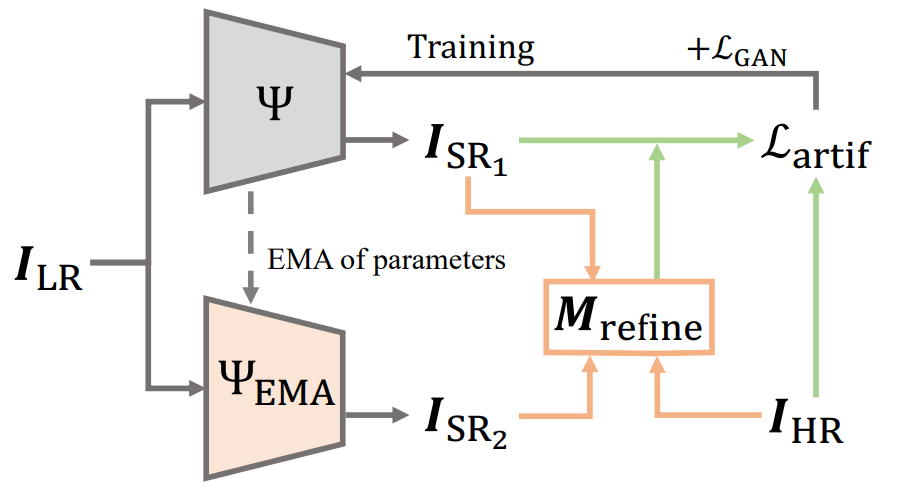
\includegraphics[width=0.7\linewidth]{LDL.png}
    \caption{Схема работы модуля LDL}
    \label{fig:LDL}
\end{figure}

\subsection{ESRGAN+LDL}
\subsubsection{ESRGAN}
В работе \cite{wang2018esrgan} предоставлена архитектура ESRGAN, являющаяся генеративно-состязательной моделью. Она состоит из генератора \ref{fig:ESRGAN} и дискриминатора. По сравнению с базовой моделью SRGAN \cite{SRGAN} ESRGAN избавили от BatchNorm и изменили функцию потерь для дискриминатора - на relativistic loss \ref{fig:rel_loss}, суть которого в следующем: заложить в модель сравнивать фальшивые изображения с настоящими, а не рассматривать каждое изображение отдельно.
В работе \cite{LDL2022} используется архитектура ESRGAN вместе с модулем LDL (см. рис. \ref{fig:LDL}), направленным на снижение частоты генерации артефактов. Рассмотрим его структуру ниже.


Целью данного исследования является создание попиксельной карты артефактов для изображения $I_{SR}$, полученного методом дистанционного зондирования. Предлагаемый метод использует как локальную, так и глобальную дисперсию, чтобы учесть влияние артефактов на высокочастотные компоненты изображения.

\subsubsection{Locally Discriminative Learning (\textbf{LDL})}

Для изображения $I_{SR}$, полученного с помощью дистанционного зондирования, целью является создание попиксельной карты $M \in \mathbb{R}^{H \times W \times 1}$, где $M(i,j) \in [0,1]$ указывает на вероятность того, что пиксель $(i,j)$ в $I_{SR}$ является артефактом. 

\subsubsection{Выделение высокочастотной составляющей}

Так как артефакты и детали являются высокочастотными компонентами изображения, и сглаженная область позволяет лучше восстановить сеть, вычисляется разница между изображением высокого разрешения $I_{HR}$ и результатом суперразрешения $I_{SR}$ для выделения высокочастотной составляющей:

$$
R = I_{HR} - I_{SR}
$$

Как показано в 3 столбце рис. \ref{fig:LDL_samples} гладких областях невязки относительно малы, в то время как в областях с высокой детализацией они велики.

\begin{figure}
    \centering
    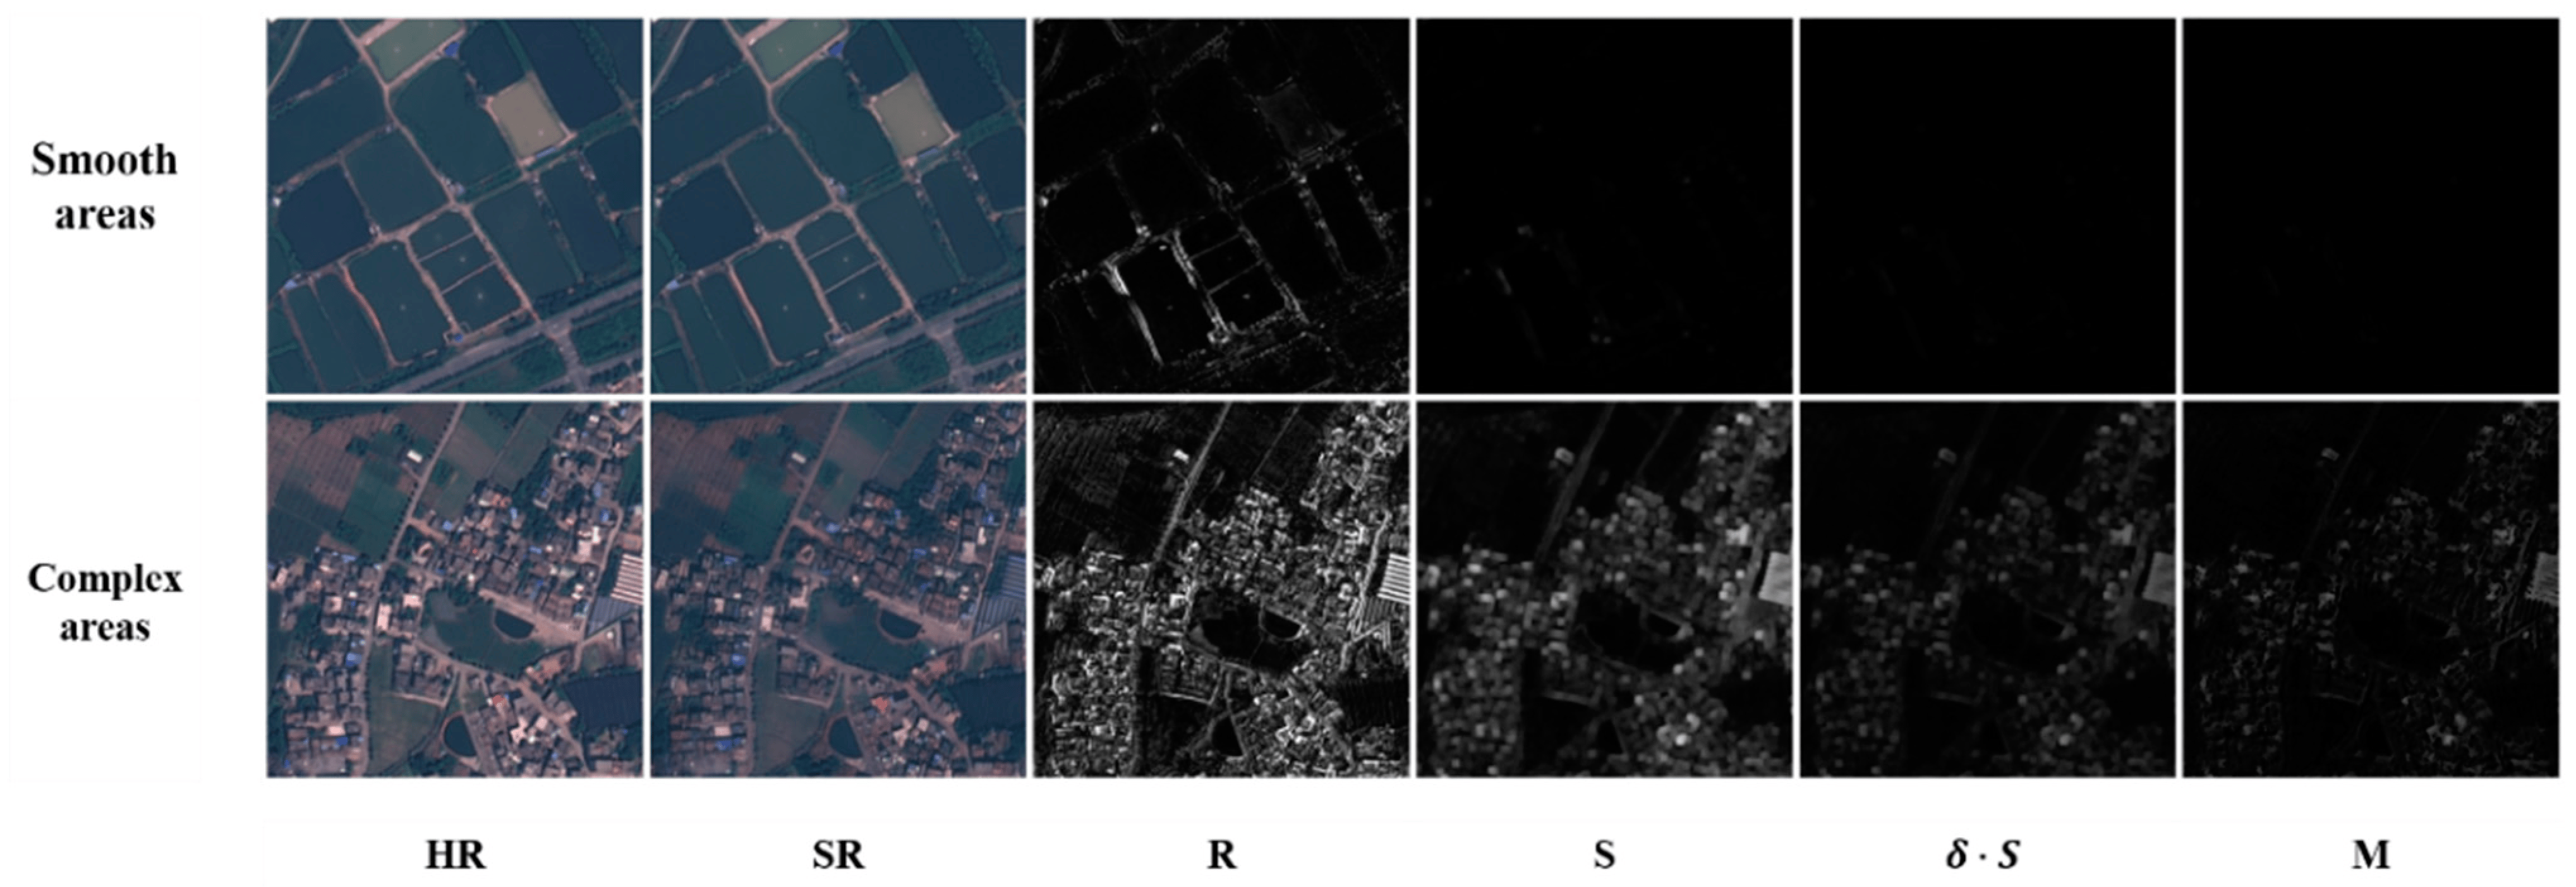
\includegraphics[width=0.7\linewidth]{LDL_samples.png}
    \caption{Визуализация процесса создания карт вероятности артефактов. HR, SR, R, S, $\delta$ · S и M представляют собой выходные данные модели GAN, изображение HR, карту остатков для расчетов HR и SR, карту локальной дисперсии, скорректированную карту локальной дисперсии и карту вероятности для артефактов соответственно.}
    \label{fig:LDL_samples}
\end{figure}

\subsubsection{Локальная дисперсия}

Для расчета вероятности наличия артефактов вводится локальная дисперсия $S$ остатков $R$:

$$
S(i,j) = \frac{1}{(n+1)^2} \sum_{x=i-\frac{n}{2}}^{i+\frac{n}{2}} \sum_{y=j-\frac{n}{2}}^{j+\frac{n}{2}} (R(x,y) - \mu)
$$

Где $\mu$ - это среднее значение в окрестности размера $n$:

$$
\mu = \frac{1}{(n+1)} \sum_{x=i-\frac{n}{2}}^{i+\frac{n}{2}} \sum_{y=j-\frac{n}{2}} R(x,y)
$$

\subsubsection{Глобальная дисперсия}

Как показано в 4 столбце рис. \ref{fig:LDL_samples}, локальная дисперсия не учитывает глобальную информацию, поэтому дополнительно вычисляется глобальная дисперсия:

$$
\delta = \left(\text{var}(R)\right)^{\frac{1}{\alpha}}
$$

Где $\alpha$ - весовой коэффициент. В экспериментах установлено, что $\alpha = 1/4$.

\subsubsection{Использование экспоненциальной скользящей средней модели (EMA)}

Как видно в 5 столбце рис. \ref{fig:LDL_samples}, вероятность появления артефактов уже почти равна нулю для гладких участков, таких как сельскохозяйственные угодья. Для повышения стабильности обучения сети GAN используется подход экспоненциальной скользящей средней (EMA):

$$
W_k^{EMA} = \alpha \cdot W_{k-1}^{EMA} + (1 - \alpha) \cdot W_k
$$

Где $W_k$ - модель на $k$-ом шаге, а $W_k^{EMA}$ - скользящее среднее модели. Параметр $\alpha$ был установлен на уровне $0.999$.


Модель $W_k^{EMA}$ является более стабильной и генерирует меньше артефактов по сравнению с $W_k$. Она используется для корректировки направления градиентного спуска:

\[
I_{SR}^{EMA} = W_k^{EMA}(I_{LR}) \quad \text{и} \quad I_{SR} = W_k(I_{LR}),
\]

где $I_{LR}$ — исходное изображение низкого разрешения, $I_{SR}$ и $I_{SR}^{EMA}$ — результаты работы моделей. Для анализа ошибок вычисляются остаточные карты $R_1$ и $R_2$:

\[
R_1 = I_{HR} - I_{SR}, \quad R_2 = I_{HR} - I_{SR}^{EMA}.
\]

Если $R_1$ больше $R_2$, это указывает на неверное обновление модели. Части $R_1$, превышающие $R_2$, считаются артефактами. Итоговая карта артефактов $M$ формируется следующим образом:

$$
M(i,j) =
  \begin{cases}
    0, & \text{если } |R_1(i,j)| < |R_2(i,j)|; \\
    \delta \cdot S(i,j), & \text{если } |R_1(i,j)| \geq |R_2(i,j)|.
  \end{cases}
$$

\subsubsection{Функция потерь}
Потери артефактов $L_{art}$ вычисляются по формуле:
$$
L_{art} = \|M \cdot R_1\|_1
$$

Для повышения качества изображений использовалась сеть VGG для выделения признаков и вычисления потерь $L_p$ между картами характеристик изображений SR и HR:
$$
L_p = \sum_i \alpha_i \| VGG_i(I_{HR}) - VGG_i(I_{SR}) \|
$$
где $i$ — номер функциональной карты сети VGG, а $\alpha_i$ — вес. Были использованы карты объектов слоев 3, 4 и 5, веса которых составили $\frac{1}{4}$, $\frac{1}{4}$ и $\frac{1}{2}$ соответственно.

В отличие от SRGAN, был применен релятивистский дискриминатор, оценивающий вероятность того, что реальное изображение более реалистично, чем SR:
$$
D_R(x_r) = \sigma(D(x_r) - \mathbb{E}_{x_f}(D(x_f))) \rightarrow 1
$$
$$
D_R(x_f) = \sigma(D(x_f) - \mathbb{E}_{x_r}(D(x_r))) \rightarrow 0
$$
где $D$ — дискриминатор, $x_r$ — изображение HR, $x_f$ — изображение SR, $\sigma$ — сигмоида.

функция потерь разделена на две части: $L_G$ для генератора и $L_D$ для дискриминатора:
$$
L_G = -\mathbb{E}_{x_r}[\log(1 - D_R(x_r))] - \mathbb{E}_{x_f}[\log(D_R(x_f))]
$$
$$
L_D = -\mathbb{E}_{x_r}[\log(D_R(x_r))] - \mathbb{E}_{x_f}[\log(1 - D_R(x_f))]
$$

Для восстановления изображения использовалась потеря $L_1$:
$$
L_1 = \mathbb{E}_I \|I_{HR} - I_{SR}\|_1
$$

Итоговые потери сети представлены следующим образом:
$$
L = \lambda_1 L_1 + \lambda_2 L_p + \lambda_3 L_G + \lambda_4 L_D + \lambda_5 L_{art}
$$
где $\lambda$ — весовые коэффициенты. В данной работе использовались значения $\lambda_1=1$, $\lambda_2=1$, $\lambda_3=0.05$, $\lambda_4=1$, $\lambda_5=1$.



\begin{figure}
    \centering
    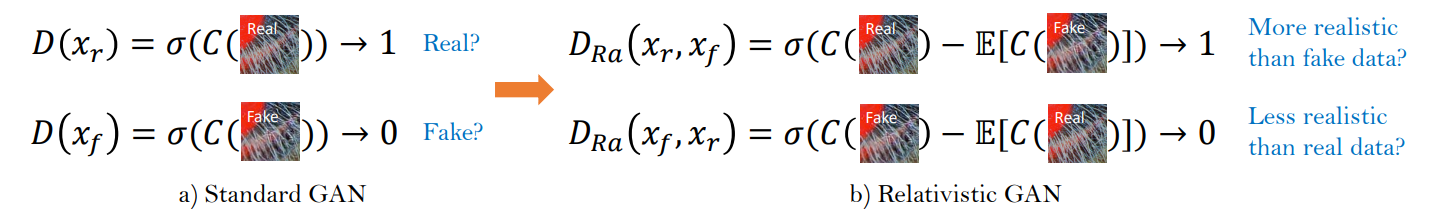
\includegraphics[width=\linewidth]{rel_loss.png}
    \caption{Отличие стандартного дискриминатора от относительного}
    \label{fig:rel_loss}
\end{figure}

\begin{figure}
  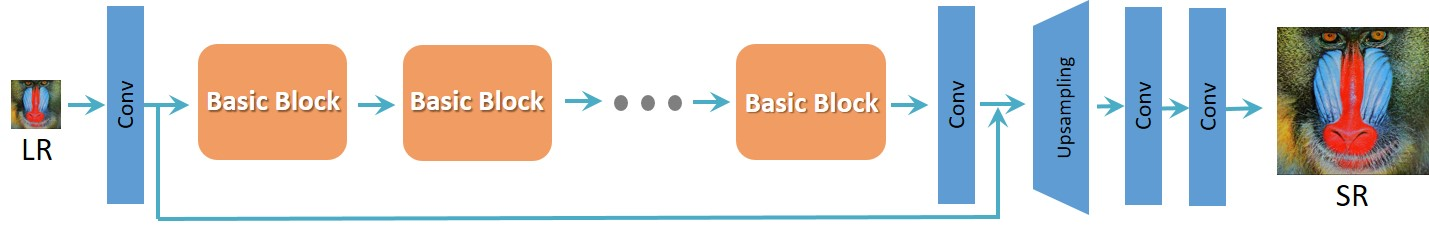
\includegraphics[width=\linewidth]{RRDN.jpg}
  \caption{Архитектура генератора ESRGAN}
  \label{fig:ESRGAN}
\end{figure}

\subsection{SwinIR}
Как показано на рис. \ref{fig:SwinIR}, архитектура SwinIR \cite{Liang2021SwinIRIR} состоит из трёх основных модулей: извлечение признаков на поверхностном и глубоком уровне (Shallow and Deep Feature Extraction), а также высококачественная (HQ) реконструкция изображений (HQ Image Reconstruction). Один и тот же модуль используется для извлечения признаков, но для разных задач применяются разные модули реконструкции.

\subsubsection{Извлечение признаков}

На этапе извлечения признаков входное изображение низкого качества $I_{LR}$ с разрешением $R^{H \times W \times 3}$ обрабатывается через свёрточные слои $HSF(\cdot)$ с ядром $3 \times 3$ для получения поверхностных признаков $F_0 \in R^{H \times W \times C}$:

$$
    F_0 = HSF(I_{LQ}),
$$

где $C$ — количество каналов. После этого глубокие признаки $F_{DF} \in R^{H \times W \times C}$ извлекаются через модуль глубокого извлечения $H_{DF}(\cdot)$, содержащий несколько блоков Swin-трансформеров (RSTB):

$$
    F_{DF} = H_{DF}(F_0).
$$

Извлечение происходит блок за блоком, где каждый $i$-й RSTB обозначается как $H_{RSTB_i}(\cdot)$:

$$
    F_i = H_{RSTB_i}(F_{i-1}), \quad F_{DF} = H_{CONV}(F_K),
$$

где $H_{CONV}$ — завершающий свёрточный слой, обеспечивающий объединение мелких и глубоких признаков для последующей реконструкции.


\subsubsection{Блок Swin-трансформера}

Блок Swin-трансформера (RSTB) содержит несколько слоёв трансформера (STL) и свёрточных слоёв. Внутри каждого блока признаки $F_{i,j}$ извлекаются через слои Swin-трансформера:

$$
    F_{i,j} = H_{STL_{i,j}}(F_{i,j-1}),
$$

где $H_{STL_{i,j}}(\cdot)$ — $j$-й уровень Swin-трансформера. Затем добавляется свёрточный слой и остаточное соединение:

$$
    F_{i,\text{out}} = H_{CONV_i}(F_{i,L}) + F_{i,0}.
$$

Эта структура позволяет объединять признаки на разных уровнях и улучшает эквивариантность трансляции SwinIR.

\subsubsection{Swin Transformer Layer}
Swin Transformer Layer (STL) \cite{liu2021swintransformerhierarchicalvision} основан на механизме многоголового самовнимания, который впервые применен в Transformer \cite{vaswani2017attentionneed}. Основные отличия STL заключаются в локальном внимании и механизме смещенного окна.

\begin{figure}
    \centering
    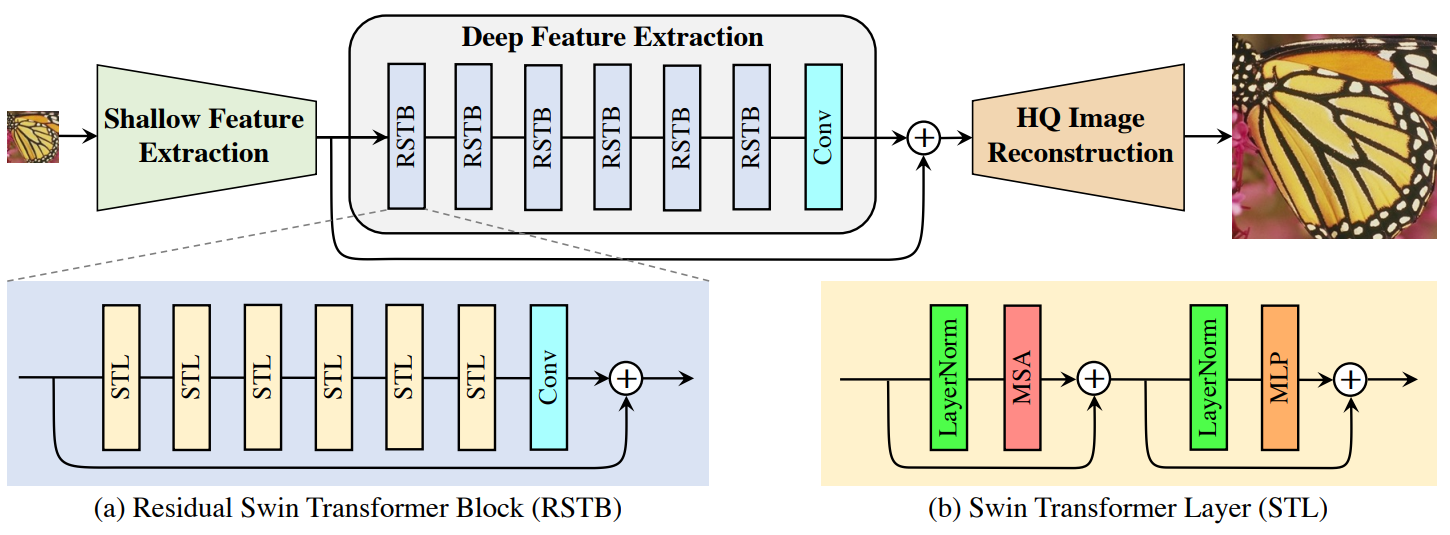
\includegraphics[width=\linewidth]{SwinIR.png}
    \caption{Архитектура SwinIR}
    \label{fig:SwinIR}
\end{figure}

\subsubsection{Механизм работы}

Для входного сигнала размером $H \times W \times C$ Swin Transformer разделяет его на неперекрывающиеся локальные окна размером $M \times M$, где количество окон — $\frac{HW}{M^2}$. Для каждого окна $X \in \mathbb{R}^{M^2 \times C}$ вычисляются запросы, ключи и значения как:
$$
    Q = XP_Q, \quad K = XP_K, \quad V = XP_V,
$$
где $P_Q$, $P_K$, $P_V$ — проекционные матрицы, общие для всех окон. Самовнимание для локальных окон рассчитывается как:
$$
    Attention(Q, K, V) = \text{SoftMax}(QK^T / \sqrt{d} + B)V,
$$
где $B$ — обучаемая относительная позиционная кодировка. Механизм многозадачного самовнимания (MSA) применяется параллельно для $h$ голов.

\subsubsection{Обработка и нормализация}

После self-attention применяется многослойный персептрон (MLP) с двумя полностью соединенными слоями и нелинейностью GELU. Также добавляется слой нормализации (LN) перед MSA и MLP. Остаточные соединения включают:
$$
    X = \text{MSA}(\text{LN}(X)) + X,
$$
$$
    X = \text{MLP}(\text{LN}(X)) + X.
$$

Для обеспечения взаимодействия между окнами используется смещенное оконное разбиение, при котором окна сдвигаются на $(\frac{M}{2}, \frac{M}{2})$ пикселей перед разбиением \cite{liu2021swintransformerhierarchicalvision}.

\subsubsection{Реконструкция изображений}

Для задачи повышения разрешения (SR) изображение высокого качества $I_{SR}$ восстанавливается путем объединения поверхностных и глубоких признаков:

$$
    I_{SR} = H_{REC}(F_0 + F_{DF}),
$$

где $H_{REC}(\cdot)$ — функция реконструкции. Мелкие признаки передают низкочастотную информацию, в то время как глубокие концентрируются на восстановлении высоких частот, что способствует стабилизированию процесса обучения.


\subsubsection{Функция потерь}

Для задачи SR параметры SwinIR оптимизируются путём минимизации потерь следующей функции:

$$
    L = \lambda_1 L_1 + \lambda_2 L_p
$$
где $L_1$ - L1 разница между восстановленным и исходным изображением, $L_p$ - perceptual loss описанный выше, $\lambda_1=1$, $\lambda_2=0.5$.

\section{Эксперименты}

\subsection{Датасет}

В данной работе для сравнения производительности ведущих архитектур использовались спутниковые снимки Массачуссетских дорог \cite{MnihThesis} с разрешением 1 пиксель на квадратный метр. Для обучения модели использвались 1170 изображений размером 1500x1500 пискелей, для валидации 50 снимков того же разрешения. Для задачи повышения разрешения в 4 раза в качестве HR изображений брались вырезанные фрагменты 256x256, LR изображения - загрубленные при помощи интерполяции и гауссовского шума изображения 64x64 пикселей.

\subsection{Детали обучения}
Архитектура модели ESRGAN состоит из генератора и дискриминатора. В данной работе использовался генератор состоящий из 23 RRDB блоков с количеством входящих каналов = 64.
В модели SwinIR используется 6 блоков RSTB и 6 слоев STL (как в иллюстрации). Во время обучения к LR-HR изображениям применялись вертикальный и горизонтальный поворот и вращение на 90 градусов. Модели обучались 400000 итераций при помощи оптимизатора Adam с шагом 1e-4. Метрики замерялись с частотой 10000 шагов.

\subsection{Метрики}
Для оценки качества сгенерированных изображений использовались следующие метрики: peak signal noise-to-ratio (PSNR), structural similarity (SSIM), Frechet inception distance (FID) и learned perceptual image patch similarity (LPIPS). PSNR определяет степень искажения, основываясь на разнице между изображениями с низким и высоким разрешением. Чем выше значение PSNR, тем выше качество изображения:
$$
    PSNR = 10 \log_{10} \frac{MAX}{MSE},
$$
где $MAX$ — максимальное значение пикселя, а $MSE$ определяется как:
$$
    MSE = \frac{1}{mn} \sum_{i=0}^{m-1} \sum_{j=0}^{n-1} [I_{SR} - I_{HR}]^2.
$$

SSIM оценивает сходство по яркости, контрастности и структуре:
$$
    SSIM(x, y) = [l(x, y)]^\alpha [c(x, y)]^\beta [s(x, y)]^\gamma.
$$
% \begin{figure}[htb]
%     \centering
%     \includegraphics[width=0.75\linewidth]{showing_ex.jpg}
%     \caption{Примеры работы упомянутых в работе архитектур в задаче повышения разрешения в 4 раза на рассмотренном выше датасете}
%     \label{fig:example}
% \end{figure}

Высокие значения PSNR и SSIM не всегда коррелируют с визуальным качеством, что требует использования дополнительных метрик, таких как FID и LPIPS.

FID измеряет расстояние между реальными и сгенерированными изображениями, используя KL дивергенцию между признаками сгенерированых и исходных изображений, которые предположительно имеют нормальное распределение:
$$
    FID(x, y) = ||\mu_x - \mu_y||^2_2 + Tr(\Sigma_x + \Sigma_y - 2 (\Sigma_x \Sigma_y)^{1/2}),
$$
где $\mu_x$, $\mu_y$ — средние значения признаков реальных и сгенерированных изображений, $\Sigma_x$, $\Sigma_y$ — их ковариации. Для замера метрики используется весь датасет или его подмножество.

LPIPS оценивает визуальное сходство, используя сеть VGG для выделения особенностей:
$$
    \sum_{l} \frac{1}{H_l W_l} \sum_{h, w} ||\omega_l \odot (x_{hw})_l - (y_{hw})_l||^2_2,
$$
где $x$, $y$ — признаки сгенерированных и реальных изображений, $\omega_l$ — весовой коэффициент для слоя $l$. Чем меньше LPIPS, тем выше качество.

% Сеть дискриминатора состоит из пяти основных блоков, где каждый блок включает в себя сверточный слой, отвечающий за извлечение объектов, сверточный слой для уменьшения размера карты объектов и функцию активации LeakyReLU.

\subsection{Результаты}
\begin{center}
\begin{tabular}{ |p{5cm}||p{2cm}|p{2cm}|p{2cm}|p{2cm}|  }
 \hline
 \multicolumn{5}{|c|}{metrics comparsion 4x} \\
 \hline
 architectures& PSNR & SSIM & LPIPS & FID\\
 \hline
 Interpolation   & 18.2             &   0.623       & 0.412          & 61.8 \\
 ESRGAN          &  23.3            &   0.696       &  0.302         & 51.2       \\
 ESRGAN + LDL    &   \textbf{24.5}  & \textbf{0.743}& 0.291          & 49.4          \\
 SwinIR          &   23.7           &   0.73        &    0.212       &      43.4     \\
 SwinIR + LDL    & 24.2    &   0.735       &    \textbf{0.176} &      \textbf{36.7}       \\
 \hline
\end{tabular}
\end{center}


% \begin{figure}
%     % \centering
%     \includegraphics[width=0.7\linewidth]{showing_ex.jpg}
%     \caption{Примеры работы упомянутых в работе архитектур в задаче повышения разрешения в 4 раза на рассмотренном выше датасете}
%     \label{fig:example}
% \end{figure}


Как видно из результатов ESRGAN показывает себя лучше в стандартных метриках SSIM и PSNR, ориентированных на попиксельное сходство, в то время как SwinIR выигрывает в метриках LPIPS и FID, выражающих более глубокое сходство восстановленного и исходного изображения.


\section{Заключение}

В данной работе был проведен сравнительный анализ передовых нейросетевых методов в области повышения пространственного разрешения для спутниковых снимков. Было показано, что LDL модуль повышает производительность модели. Рассмотрены архитектуры ESRGAN и SwinIR с применением LDL модуля для снижения частоты генерации артефактов при восстановлении изображения.

\printbibliography




\end{document}